\documentclass[10pt, a5paper]{article}
\usepackage{pdfpages}
\usepackage{parallel}
\usepackage[T2A]{fontenc}
\usepackage{ucs}
\usepackage[utf8x]{inputenc}
\usepackage[polish,english,russian]{babel}
\usepackage{hyperref}
\usepackage{rotating}
\usepackage[inner=2cm,top=1.8cm,outer=2cm,bottom=2.3cm,nohead]{geometry}
\usepackage{listings}
\usepackage{graphicx}
\usepackage{wrapfig}
\usepackage{longtable}
\usepackage{indentfirst}
\usepackage{array}
\newcolumntype{P}[1]{>{\raggedright\arraybackslash}p{#1}}
\frenchspacing
\usepackage{fixltx2e} %text sub- and superscripts
\usepackage{icomma} % коскі ў матэматычным рэжыме
\PreloadUnicodePage{4}

\newcommand{\longpage}{\enlargethispage{\baselineskip}}
\newcommand{\shortpage}{\enlargethispage{-\baselineskip}}

\def\switchlang#1{\expandafter\csname switchlang#1\endcsname}
\def\switchlangbe{
\let\saverefname=\refname%
\def\refname{Літаратура}%
\def\figurename{Іл.}%
}
\def\switchlangen{
\let\saverefname=\refname%
\def\refname{References}%
\def\figurename{Fig.}%
}
\def\switchlangru{
\let\saverefname=\refname%
\let\savefigurename=\figurename%
\def\refname{Литература}%
\def\figurename{Рис.}%
}

\hyphenation{admi-ni-stra-tive}
\hyphenation{ex-pe-ri-ence}
\hyphenation{fle-xi-bi-li-ty}
\hyphenation{Py-thon}
\hyphenation{ma-the-ma-ti-cal}
\hyphenation{re-ported}
\hyphenation{imp-le-menta-tions}
\hyphenation{pro-vides}
\hyphenation{en-gi-neering}
\hyphenation{com-pa-ti-bi-li-ty}
\hyphenation{im-pos-sible}
\hyphenation{desk-top}
\hyphenation{elec-tro-nic}
\hyphenation{com-pa-ny}
\hyphenation{de-ve-lop-ment}
\hyphenation{de-ve-loping}
\hyphenation{de-ve-lop}
\hyphenation{da-ta-ba-se}
\hyphenation{plat-forms}
\hyphenation{or-ga-ni-za-tion}
\hyphenation{pro-gramming}
\hyphenation{in-stru-ments}
\hyphenation{Li-nux}
\hyphenation{sour-ce}
\hyphenation{en-vi-ron-ment}
\hyphenation{Te-le-pathy}
\hyphenation{Li-nux-ov-ka}
\hyphenation{Open-BSD}
\hyphenation{Free-BSD}
\hyphenation{men-ti-on-ed}
\hyphenation{app-li-ca-tion}

\def\progref!#1!{\texttt{#1}}
\renewcommand{\arraystretch}{2} %Іначай формулы ў матрыцы зліпаюцца з лініямі
\usepackage{array}

\def\interview #1 (#2), #3, #4, #5\par{

\section[#1, #3, #4]{#1 -- #3, #4}
\def\qname{LVEE}
\def\aname{#1}
\def\q ##1\par{{\noindent \bf \qname: ##1 }\par}
\def\a{{\noindent \bf \aname: } \def\qname{L}\def\aname{#2}}
}

\def\interview* #1 (#2), #3, #4, #5\par{

\section*{#1\\{\small\rm #3, #4. #5}}

\def\qname{LVEE}
\def\aname{#1}
\def\q ##1\par{{\noindent \bf \qname: ##1 }\par}
\def\a{{\noindent \bf \aname: } \def\qname{L}\def\aname{#2}}
}

\switchlang{ru}
\begin{document}
\title{Электромиографическое распознавание движений пальцев руки человека на базе Arduino\footnote{\url{shadimx@gmail.com}, \url{http://lvee.org/ru/abstracts/245}}}
\author{Вадим Шамонин, Брест, Belarus}
\maketitle
\begin{abstract}
An open hardware project for the electromyography measurements is presented. Arduino platform is engaged in getting data from the epidermic sensors and passing them to the receiving software to detect and classify muscle activity. Results of fingers movements recognition are presented for two sensors placement approaches.
\end{abstract}
\subsection*{Введение}

В настоящее время разрабатывается большое количество устройств, позволяющих использовать пальцы рук в качестве источника управляющих сигналов. Все их можно разделить на три категории:

\begin{itemize}
  \item механические манипуляторы, повторяющие движения человеческой руки;
  \item взаимодействие с объектами в системах виртуальной и/или дополненной реальности;
  \item мониторинг биологических параметров организма.
\end{itemize}

Применения электромиографического метода (ЭМГ) для этого круга задач делает возможным не только распознавание степени сгибания пальцев с высокой точностью, но также позволяет использовать полученные данные для выявления медицинских отклонений пациента. ЭМГ также предоставляет новые возможности в области реабилитации после инсульта. К примеру, антропоморфная робототехника, применяемая в медицине, позволяет регулярно разгибать руку у человека, который в результате болезни потерял такую возможность (это называется нейрореабилитацией, и применяется в том числе после инсультов и нейротравм).

\begin{center}

\begin{figure}[h!]
  \centering
  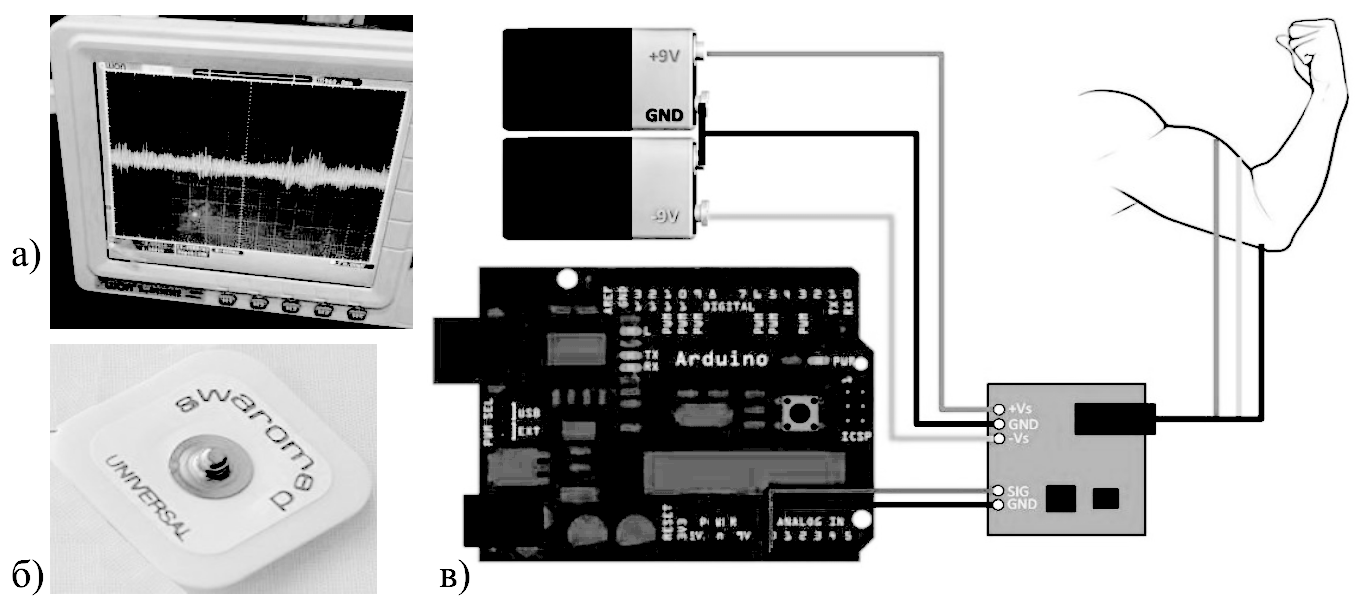
\includegraphics[width=9cm]{Shamonin1.PNG}
  \caption{Используемые накожные электроды Ag/AgCl (а), визуализация сигналов с них, снятых без усиления (б) и схема подключения усилителя (в)}
  \label{Shamonin1}

\end{figure}

\end{center}


\subsection*{Аппаратная платформа и особенности реализации}

Разработанное устройство построено на основе платформы Arduino. Проект разрабатывается как open hardware, наработки доступны по адресу \url{https://github.com/shadimx}.

При помощи неё данные обрабатываются при подключении к ПК. Электрическую активность мышц при помощи накожных Ag-электродов, широко используемых в медицинских целях при записи ЭКГ (рис. ~\ref{Shamonin1}). Для более точного выявления биопотенциалов используется специализированный OpenHardware-модуль цифрового усиления сигналов для Arduino — muscle sencor v3 от sparkfun (рис. ~\ref{Shamonin1}).

\subsection*{Особенности измерений}

Для решения задачи распознавания движений пальцами важную роль играет методика регистрации ЭМГ. В работе рассмотрены 2 методики регистрации сигналов при использовании неинвазивной ЭМГ.

В рамках 1-й методики положения №4 и №5, также как и №6 и №7 (рис. ~\ref{Shamonin2}) регистрировались одним электродом. Сигналы записывались относительно канала “Reference”, положение которого выбиралось на участке выше локтя, на котором отсутствуют сокращения мышц при движении пальцами. Электрод канала “Ground” располагался в районе плечевого сустава. В рамках 2-й методики те же положения регистрировались отдельными электродами, при положении электродов каналов “Reference” и “Ground” таком же, как в 1-й методике. Кроме того, снималось также 5 дифференциальных каналов между положениями 1 и 2; 3 и 4; 5 и 6; 7 и 8; 9 и 10. В результате методика с использованием дифференциальных каналов позволила улучшить отношение сингал/шум, что обеспечило существенно лучшее качество распознавания движений классификатором (рис. ~\ref{Shamonin2}). Отметим, что использование некоторых каналов не улучшает работу классификатора. Для 2-й методики достаточно использовать 5 дифференциальных и 2 отдельных канала.

\begin{center}
\begin{figure}[h!]
  \centering
  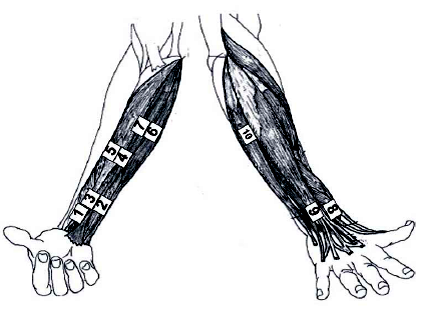
\includegraphics[width=6cm]{Shamonin2.png}
  \caption{Положение электродов при регистрации ЭМГ}
  \label{Shamonin2}

\end{figure}

\end{center}

Практическим методом была установлена взаимосвязь амплитуды получаемого сигнала на конкретном участке мышцы от степени сгибания пальцев руки.

В результате проверки выбранных методик измерения были получены 65\% и 95\% вероятности правильного определения сгибания пальца для 1-й и 2-й методик соответственно (рис. ~\ref{Shamonin3}). Время работы наиболее удовлетворительного алгоритма классификации составляет 0,5 мс, что позволяет применять его в режиме реального времени.
\begin{center}

\begin{figure}[h!]
  \centering
  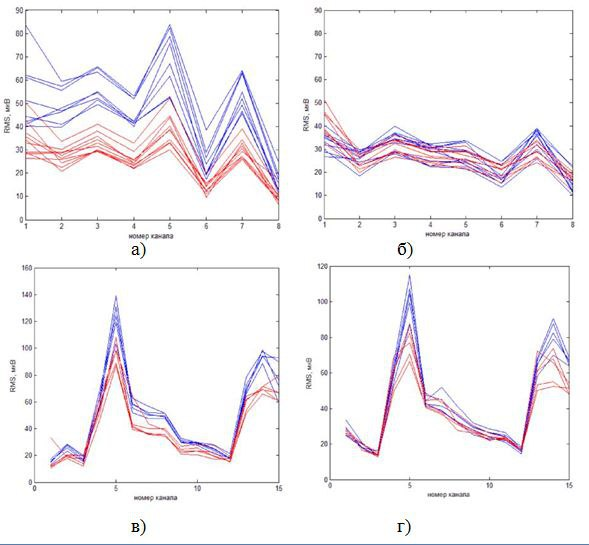
\includegraphics[width=8cm]{Shamonin3.jpg}
\caption{Примеры распознавания движений мизинца (а, в) и указательного пальца (б, г) в рамках 1-й (а, б) и 2-й (в, г) методик}
  
  \label{Shamonin3}

\end{figure}

\end{center}

\begin{thebibliography}{20}

\bibitem{shamonin-1} Muscle Sensor v3 Kit \url{https://www.sparkfun.com/products/retired/11776}

\end{thebibliography}

\end{document}
